\documentclass[a4paper,14pt, unknownkeysallowed]{extreport}

\usepackage{cmap} % Улучшенный поиск русских слов в полученном pdf-файле
\usepackage[T2A]{fontenc} % Поддержка русских букв
\usepackage[utf8x]{inputenc} % Кодировка utf8
\usepackage[english,russian]{babel} % Языки: русский, английский
\usepackage{enumitem}


\usepackage{threeparttable}

\usepackage[14pt]{extsizes}

\usepackage{caption}
\captionsetup{labelsep=endash}  
\captionsetup[figure]{name={Рисунок}}

% \usepackage{ctable}
% \captionsetup[table]{justification=raggedleft,singlelinecheck=off}

\usepackage{amsmath}

\usepackage{geometry}
\geometry{left=30mm}
\geometry{right=10mm}
\geometry{top=20mm}
\geometry{bottom=20mm}

\usepackage{titlesec}
\titleformat{\section}
	{\normalsize\bfseries}
	{\thesection}
	{1em}{}
\titlespacing*{\chapter}{0pt}{-30pt}{8pt}
\titlespacing*{\section}{\parindent}{*4}{*4}
\titlespacing*{\subsection}{\parindent}{*4}{*4}

\usepackage{setspace}
\onehalfspacing% Полуторный интервал

\frenchspacing
\usepackage{indentfirst} % Красная строка

\usepackage{titlesec}
\titleformat{\chapter}{\LARGE\bfseries}{\thechapter}{20pt}{\LARGE\bfseries}
\titleformat{\section}{\Large\bfseries}{\thesection}{20pt}{\Large\bfseries}

\usepackage{multirow}
\usepackage{listings}
\usepackage{xcolor}

% Для листинга кода:
\lstset{%
	language=c++,   					% выбор языка для подсветки	
	basicstyle=\small\sffamily,			% размер и начертание шрифта для подсветки кода
	numbers=left,						% где поставить нумерацию строк (слева\справа)
	numberstyle=\tiny,		     		% размер шрифта для номеров строк
	stepnumber=1,						% размер шага между двумя номерами строк
	numbersep=5pt,						% как далеко отстоят номера строк от подсвечиваемого кода
	frame=single,						% рисовать рамку вокруг кода
	tabsize=4,							% размер табуляции по умолчанию равен 4 пробелам
	captionpos=t,						% позиция заголовка вверху [t] или внизу [b]
	breaklines=true,					
	breakatwhitespace=true,				% переносить строки только если есть пробел
	backgroundcolor=\color{white},
	basicstyle=\footnotesize\ttfamily,
	keywordstyle=\color{blue},
	stringstyle=\color{red},
	commentstyle=\color{gray}
	showspaces=false,
    showstringspaces=false
}


\usepackage{pgfplots}
\usetikzlibrary{datavisualization}
\usetikzlibrary{datavisualization.formats.functions}




\usepackage{graphicx}
\graphicspath{ {images/} }
\newcommand{\img}[3] {
	\begin{figure}[h!]
		\center{\includegraphics[height=#1]{img/#2}}
		\caption{#3}
		\label{img:#2}
	\end{figure}
}


\usepackage[justification=centering]{caption} % Настройка подписей float объектов

\usepackage[unicode,pdftex]{hyperref} % Ссылки в pdf
\hypersetup{hidelinks}

\usepackage{csvsimple}

\newcommand{\code}[1]{\texttt{#1}}

\usepackage{longtable}

\usepackage{array}
\usepackage{booktabs}
\usepackage{floatrow}

\floatsetup[longtable]{LTcapwidth=table}

\def\UrlBreaks{\do\/\do-\do\_}

\makeatletter
\renewcommand*\l@chapter[2]{%
  \ifnum \c@tocdepth >\m@ne
    \addpenalty{-\@highpenalty}%
    \vskip 1.0em \@plus\p@
    \setlength\@tempdima{1.5em}%
    \begingroup
      \parindent \z@ \rightskip \@pnumwidth
      \parfillskip -\@pnumwidth
      \leavevmode \bfseries
      \advance\leftskip\@tempdima
      \hskip -\leftskip
      #1\nobreak\normalfont\leaders\hbox{$\m@th
        \mkern \@dotsep mu\hbox{.}\mkern \@dotsep
        mu$}\hfill\nobreak\hb@xt@\@pnumwidth{\hss #2}\par
      \penalty\@highpenalty
    \endgroup
  \fi}
\makeatother

\begin{document}



\setcounter{page}{4}
\renewcommand{\contentsname}{Содержание} 
\tableofcontents


\setcounter{page}{5}
\chapter{Введение}
\addcontentsline{toc}{chapter}{Введение}

TODO: придумать введение





\chapter{Аналитическая часть}

\section[Анализ алгоритмов создания отражений]{Анализ алгоритмов визуализации}



При построении реалистичного изображения необходимо с полированными поверхностями необходимо визуализировать отражения света от тел.
Существуют множество подходов для создания реалистичных изображений:
\begin{enumerate}
	\item Трассировка световых лучей(Ray tracing)
	\item Отображения отражений(Reflection mapping)
	\item Трассировка лучей в пространстве изображения(Screen-space reflections)
\end{enumerate}



\begin{figure}[h]
	\centering
	\includegraphics{global_model_light.png}
	\caption{Пример трассировки луча}
	\label{fig:global_model_light}
\end{figure} 

Заметим что на рисунке \ref{fig:global_model_light}  призма, загороженная от наблюдателя параллелипипедом,становится видимой из-за отражения в сфере.
Точка 5 видима, так как отражается от обратной стороны параллелипипеда в точке 4 к точке 3 на сфере, а затем к наблюдателю.
Таким образом, при создании глобальной модели освещения, алгоритмы , основанные на удалении невидимых поверхностей не будут давать изображения необходимого качества.


\subsection{Алгоритм трассировки лучей}
\textbf{Основная идея алгоритма - симуляция физического процесса прохождения света} \newline
В реальной жизни объекты являются видимыми, в случае если они отражают свет от источника, после чего данные лучи света попадают в человеческий глаз.Аналогичная идея заложена в данном способе создания изображения - необходимо отследить движение лучей света.
Заметим, что отслеживать путь всех лучей света не стоит, так как это неэффективно, при построении изображения внимаение следует уделять объектам видимыми со стороны наблюдателя.
В таком случае можно отслеживать лучи света, исходящие из точки наблюдения, т.е. производить трассировку лучей в обратном направлении.В нашем случае лучи стоит проводить через центры пикселей изображения,
считается ,что наблюдатель находится на бесконечности, из-за чего все лучи параллельны оси OZ.\cite{Rodgers}

\begin{figure}[h]
	\centering
	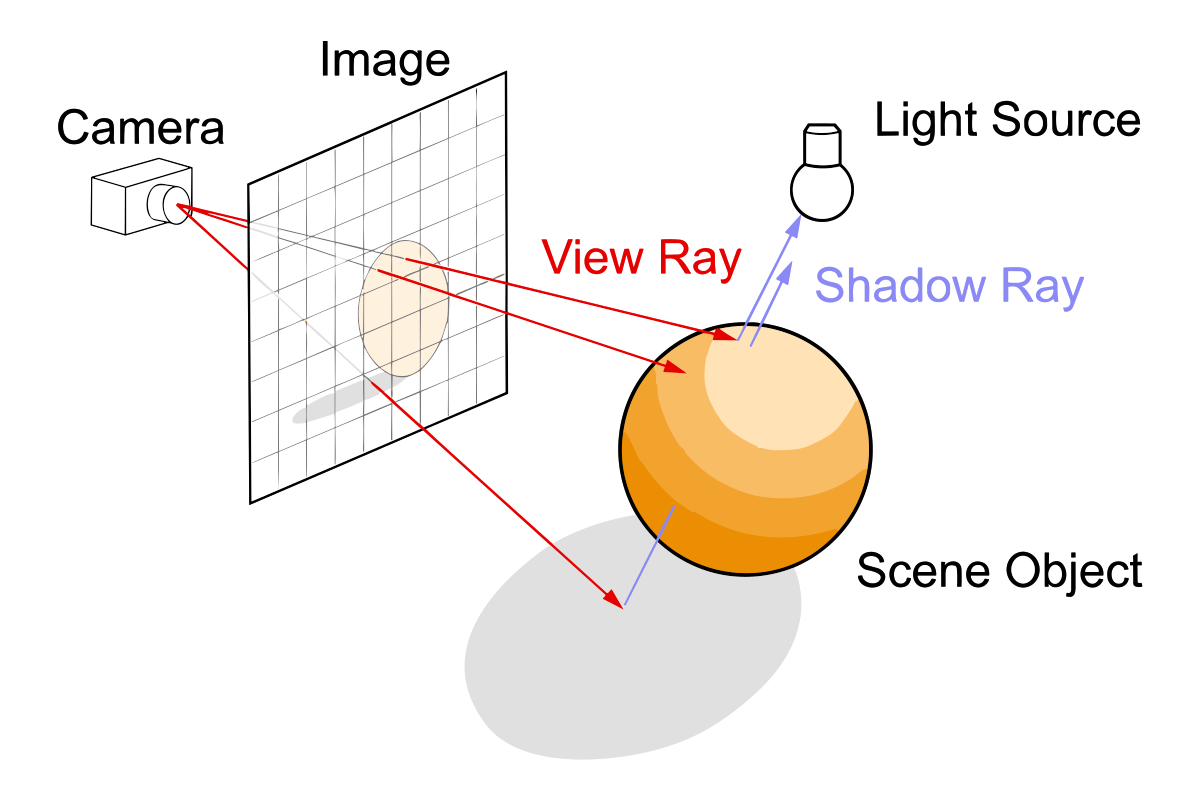
\includegraphics[scale=0.4]{ray_tracing.jpg}
	\caption{Пример трассировки луча}
	\label{fig:alg_ray_tracing}
\end{figure} 

Первые работы принадлежат Уиттеду и Кэю.Алгоритм Уиттеда более общий и часто используется.[Роджерс с.438]
Уиттед пользуется моделью , в которой диффузная и зеркальная составляющие отражения расчитываются подобно локальной модели.
Диффузное отражения одинаково во всех направлениях, так что наибольшую проблему представляет расчет зеркальных отражений.\cite{Rodgers}

\begin{figure}[h]
	\centering
	\includegraphics{global_reflections.jpg}
	\caption{Расчет зеркального отражения луча в алгоритме Уиттеда}
	\label{fig:global_reflections}
\end{figure} 

На рисунке  \ref{fig:global_reflections} луч \textbf{V} падает на поверхность в точку \textbf{Q}, после чего отражается в направлении \textbf{r} и преломляется
в направлении \textbf{p}.
В данном случае:
\begin{enumerate}
	\item $I_t$ - интенсивность света, падающего в точку \textbf{p}.
	\item $\eta$ - показатели преломелния сред(влияют на направление преломленного луча)
	\item $S$,$R$ - полученные вектора наблюдения и отражения
	\item $L_j$ - Вектор к источнику света $j$

\end{enumerate}

Тогда наблюдаемая интенсивность \textbf{I} выражается формулой:
\begin{equation} 
	I = k_aI_a + k_d \sum_{j} I_{l_j}(\hat{n} * \hat{L_j}) + k_s \sum_{j} I_{l_j}(\hat{S} * \hat{R_j})^n + k_sI_s + k_tI_t
	\label{eq:intensivity}
\end{equation}

В формуле \ref{eq:intensivity} соответственно означают:
\begin{enumerate}
	\item $k_a,k_d,k_s$ - коэффициенты рассеянного, диффузного,зеркального отражения соответственно
	\item $k_t$ - коэффициент пропускания
	\item $n$ - cтепень пространственного распределения Фонга
\end{enumerate}
В данном случае знак $ \hat{} $  означает что данный вектор нормализован
Значения коэффициентов определяются внешней средой и могут, а также могут определяться длинной волн света
Таким образом возможно посчитать интенсивность света для отраженной и преломленной части луча.
После чего полученные вычисления необходимо выполнить еще раз для отраженного и преломелнного луча и т.д.(Todo:были правила про верное написание т.д. - прочитать)
и сложить полученные интенсивности.
Теоритически свет может отражаться бесконечно, так что стоит ограничить число рассматриваемых отражений либо определенным числом,
либо не рассматривать лучи с интенсивностью меньше определенного значения
Таким образом данный алгоритм имеет асимптотику $O(N*C*2^{K})$ , где \textbf{N} - количество тел,\textbf{C} - количество испускаемых лучей,
\textbf{K} - количество рассматриваемых отражений света. \cite{Rodgers}


\textbf{Достоинства алгоритма}:
\begin{enumerate}
	\item Создание реалистичных изображений
	\item Возможность наблюдения физических явлений, так как алгоритм симулирует поведение света в реальной жизни
\end{enumerate}


\textbf{Недостатки алгоритма}:
\begin{enumerate}
	\item Время работы
	\item Количество требуемой памяти, так как в памяти необходимо хранить все отраженные и преломленные лучи, полученные при предыдущих расчетах
\end{enumerate}


\subsection{Трассировка лучей в пространстве изображения}
\textbf{Основная идея алгоритма - симуляция физического процесса прохождения света, рассматривая только видимые объекты} \newline
Обычно при необходимости расчета отражений и теней уже известны объекты, которые находятся на сцене.При использовании SSR(Screen-space reflections),используется информация о имеющихся
объектов из-за чего трудозатраты на создание изображения заметно сокращаются.
Перед началом алгоритма требуется информация о:
\begin{enumerate}
	\item Координата Z наиближайшей к наблюдателю поверхности
	\item Нормаль данной поверхности
\end{enumerate}

\begin{figure}[h]
	\centering
	\includegraphics{SSR_data_flow.png}
	\caption{Поток данных при использовании SSR}
	\label{fig:SSR_data_flow}
\end{figure} 

До началы работы самого алгоритма необходимо подготовить данные, что происходит в два этапа:
\begin{enumerate}
	\item Геометрический проход(Geometry pass)
	\item Световой проход(Lightning pass)
\end{enumerate}

На картинке \ref{fig:SSR_data_flow} используется понятие \textbf{G-buffer}, данный буффер содержит все необходимые данные для начала работы алгоритма,данные для данного буфера
будут получены после геометрческого прохода. В общем случае он содержит для каждого пикселя:
\begin{enumerate}
	\item Нормали к видимым поверхностям
	\item Значение z наиближайшей видимой фигуры
	\item Свойства материалов, значимые для трассировки света(коэффициенты диффузного и зеркального отражения)
\end{enumerate}
При световом проходе для каждого пикселя выбираются источники,которые влияют на его интенсивность
Работа SSR аналогична работе алгоритма \textbf{Ray tracing},однако информация о видимых объектах уже получена и будут рассматриваться только они.
Из-за этого,если часть объекта не видима то изображение будет не корректным, как ,например, на картинке \ref{fig:SSR_fail}.
\begin{figure}[h]
	\centering
	\includegraphics[scale=0.4]{SSR_fail.jpg}
	\caption{Некорректный расчет отражений при использовании SSR}
	\label{fig:SSR_fail}
\end{figure} 

\textbf{Достоинства алгоритма}:
\begin{enumerate}
	\item Меньшее число трудозатрат,чем при использовании алгоритма трассировки лучей
\end{enumerate}

\textbf{Недостатки алгоритма}:
\begin{enumerate}
	\item При наличии невидимых для наблюдателя частей объектов в отражении изображение будет некорректным
	\item Искажение геометрии при генерации изображений
\end{enumerate}

\subsection{Отображение отражений}
\textbf{Основная идея - создание текстуры я уже просчитанными отражениями,после чего наложить ее на зеркальный предмет} \newline
Для того чтобы получить текстуру,достаточно предварительно расчитать изображения в 6 направлениях для необходимого объекта, получив кубическую карту, ее пример представлен на картинке \ref{fig:cube_maps}
\begin{figure}[h]
	\centering
	\includegraphics[scale=0.4]{cube_maps}
	\caption{Пример кубической карты(cube maps)}
	\label{fig:cube_maps}
\end{figure}
\newline
Например для объекта \ref{fig:cube_maps_real}, будет получена карта \ref{fig:cube_maps_real_example}


\begin{figure}[h]
	\centering
	\includegraphics[scale=0.4]{cube_maps_real}
	\caption{Положение объекта для построения карты}
	\label{fig:cube_maps_real}
\end{figure}


\begin{figure}[h]
	\centering
	\includegraphics[scale=0.4]{cube_maps_real_example}
	\caption{Полученная кубическая карта}
	\label{fig:cube_maps_real_example}
\end{figure}


Однако динамически обновлять данную текстуру очень трудозатратно(необходимо отрсиовать сцену 6 раз).

\textbf{Достоинства алгоритма}:
\begin{enumerate}
	\item При статических текстурах не тратится время на расчет отражений и теней
\end{enumerate}

\textbf{Недостатки алгоритма}:
\begin{enumerate}
	\item Расчет изменяющейся картинки очень трудозатратен
\end{enumerate}

\subsection{Выбор оптимального алгоритма}
При реализации отражений примитивов точность их представления играет решающую роль.Единственный алгоритм из рассмотренных, который позволяет представить максимально
реалистичное изображение - \textbf{Алгоритм трассировки лучей}.Так как выбранные примитивы простые, то при использовании данного алгоритма вычислительная
сложность не будет являться критически высокой.











%\begin{thebibliography}{9}
	%\bibitem{bib1}
	%Демин А. Ю., Основы компьютерной графики [Электронный ресурс] // Томс, Томский политехнический университет. 2011. URL: \url{https://portal.tpu.ru/SHARED/j/JBOLOTOVA/academic/ComputerGraphics/CGStudyBook.pdf}.
	%\bibitem{bib2}
	%Набережнов Г. М., Максимов, Н. Н. Трехмерное моделирование полигональными сетками [Электронный ресурс] // Казань, Казанский государственный технический университет им. А.Н.Туполева. 2008. URL: \url{https://studfile.net/preview/7335496/}.
	%bibitem{bib3}
	%Польский С. В., Компьютерная графика [Электронный ресурс] // Москва, Московский государственный университет леса. 2008. URL: \url{https://mf.bmstu.ru/info/faculty/kf/caf/k3/subjects/Computer_graphics/materials/CG_RGR.pdf}.
	%\bibitem{bib4}
	%Селянкин В. В., Алгоритмы трехмерной графики [Электронный ресурс] // Таганрог, Южный федеральный университет. 2007. URL: \url{http://ntb.tgn.sfedu.ru/UML/UML_4112.pdf}.
	%\bibitem{bib5}
	%Rogers D., Adams J., Matematical Elements for Computer Graphics [Электронный ресурс] // Аннаполис, United States Naval Academy. 1989. URL: \url{https://itslearningakarmazyan.files.wordpress.com/2015/08/rodzhers_adams.pdf}.
	%\bibitem{bib6} Eck D., Introduction to Computer Graphics [Электронный ресурс] // Нью-Йорк, Hobart and William Smith Colleges. 2021. URL: \url{https://math.hws.edu/eck/cs424/downloads/graphicsbook-linked.pdf}.
	%\bibitem{bib7}
	%Programming Languages -- C++ [Электронный ресурс] // 2020. URL: \url{https://isocpp.org/files/papers/N4860.pdf}.
	%\bibitem{bib8}
	%Qt Documentation [Электронный ресурс] // URL: \url{https://doc.qt.io/qt-6/}.
	%\bibitem{bib9}
	%OpenMP Specifications [Электронный ресурс] // URL: \url{https://www.openmp.org/specifications/}.
%\end{thebibliography}


\begin{thebibliography}{9}
	\bibitem{Rodgers}
	Роджерс Д. Алгоритмические основы машинной графики. - 1-е изд. - Москва: Мир, 1989. - 512 с.
	
	
\end{thebibliography}

\addcontentsline{toc}{chapter}{Список литературы}



\end{document}